% Created 2016-08-02 Tue 10:54
\documentclass[11pt]{article}
\usepackage[utf8]{inputenc}
\usepackage[T1]{fontenc}
\usepackage{fixltx2e}
\usepackage{graphicx}
\usepackage{longtable}
\usepackage{float}
\usepackage{wrapfig}
\usepackage{rotating}
\usepackage[normalem]{ulem}
\usepackage{amsmath}
\usepackage{textcomp}
\usepackage{marvosym}
\usepackage{wasysym}
\usepackage{amssymb}
\usepackage{hyperref}
\tolerance=1000
\author{Nathan}
\date{\today}
\title{gravi\_ideas}
\hypersetup{
  pdfkeywords={},
  pdfsubject={},
  pdfcreator={Emacs 25.1.50.2 (Org mode 8.2.10)}}
\begin{document}

\maketitle
\tableofcontents

\clearpage 

\section{Lifting mechanisms}
\label{sec-1}

One possible solution to our problems could be to introduce a lifting mechanism this would allow us to tare each load cell before a reading, making it 
more likely that we would received a correct reading. 

Any solution which uses a lift would require us to have a dual table system: 


\subsection{Linear Actuator}
\label{sec-1-1}

\href{http://www.instructables.com/id/Electric-Height-Adjustable-Desk/?ALLSTEPS}{Drawing inspiration from this example} we could attempt to make use of the hollow legs in the current
tables by inserting actuators in them. 

Whilst this would make for a nice setup that could be automated, it does become a little more complex 
and does introduce a few areas of concern. However these devices are generally very reliable. 
\begin{figure}[htb]
\centering
\includegraphics[width=.9\linewidth]{./images/linear.png}
\caption{\label{fig:Linear-Actuator}Linear actuators at four corners to lift bench}
\end{figure}

\subsubsection{Alternate design}
\label{sec-1-1-1}

Rather than lifting the plants each time, it might be more prudent to lift the scales themselves rather than the 
plants each time. It would generally be less load on the actuators, however 
\begin{figure}[htb]
\centering
\includegraphics[width=200px]{./images/linear2.png}
\caption{\label{fig:Linear-Actuator}Linear actuators at four corners to lift bench}
\end{figure}


\subsubsection{Choice of Actuator}
\label{sec-1-1-2}

If we assume that each bench will have up-to 8 load cells on it, each with a max of 10kg each (including itself) 
then we would need a device capable of 80kg force

\begin{center}
\begin{tabular}{rlll}
Option & Price & Potential Lift & Range\\
1 & £89.77 & 28.1N & 48mm\\
2 & £25.55 & 43N & 10mm\\
3 & £174.27 & 500N & 50mm\\
\end{tabular}
\end{center}

I would have assumed that option 2 could have a lot of potential as we really only need a minimum lift 
from the surface of the load cells in order to perform a tare function. 

I've selected option 1 as a mid-priced option and option 3 as a "if we were considering heavier plants." 
\begin{enumerate}
\item Option 1:
\label{sec-1-1-2-1}

\begin{itemize}
\item \url{http://uk.rs-online.com/web/p/electric-linear-actuators/4540990/?origin=PSF_421233|cav}

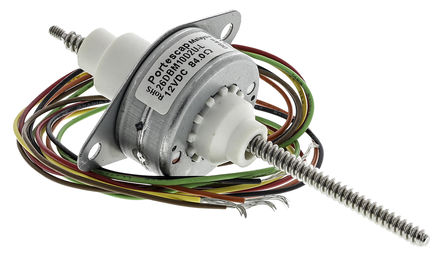
\includegraphics[width=150px]{./images/act1.jpg}
\end{itemize}


\item Option 2:
\label{sec-1-1-2-2}

\begin{itemize}
\item \url{http://uk.rs-online.com/web/p/electric-linear-actuators/4947234/}

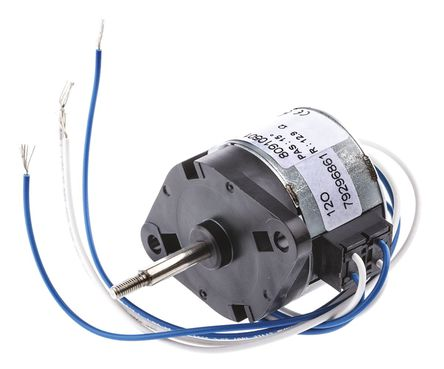
\includegraphics[width=150px]{./images/act2.jpg}
\end{itemize}

\item Option 3:
\label{sec-1-1-2-3}

\begin{itemize}
\item \url{http://uk.rs-online.com/web/p/electric-linear-actuators/7643477/}

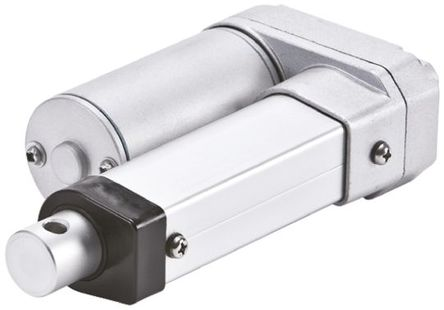
\includegraphics[width=150px]{./images/act3.jpg}
\end{itemize}
\end{enumerate}


\subsection{Scissor Jack}
\label{sec-1-2}

A scissor style jack could be a potential solution as it would probably be the lowest cost (initially) solution, a 
jack could cost us under £15. The downside being that this is a semi-manual solution were we would have to hand wind
the jack up and down for each bench

However it is feasible that a balance could be reliable to +- 2\textasciitilde{}\% for the first 3 days. This could mean we just have to twice a week perform a manual taring. It would save having to 
lift by hand 120 plants. 

Although there are potential improvements which could be made to automate this process with motorized devices. 

\begin{figure}[htb]
\centering
\includegraphics[width=150px]{./images/bench2.png}
\caption{\label{fig:Scissor-Jack-2}Alternate placement making use of one scissor jack}
\end{figure}


\begin{enumerate}
\item Placement of Jack
\label{sec-1-2-0-1}
Initially I would have thought that this placement shown would be fine for the jack, where it would push from the center of 2 joint benches 
in order to successfully use one lift without any breaks. 


\begin{figure}[htb]
\centering
\includegraphics[width=150px]{./images/tables.png}
\caption{\label{fig:Jack-location}Red cross showing where the jack would be}
\end{figure}


\subsubsection{Choice of Scissor jack}
\label{sec-1-2-1}

There are a lot of retailers offering scissor jacks, as an example I have provided a link to \href{https://www.amazon.co.uk/3M-66183c-Tonne-Scissor-Jack/dp/B002NUBHAM}{Amazon} (which is one of the cheaper ones). 
It is a fairly standard item so not a problem to get a hold off. 

\subsubsection{Alternate solution: Two Jack}
\label{sec-1-2-2}
Another possible solution is to use two individual jacks in order to push from either side at the same time to better stable.
\begin{figure}[htb]
\centering
\includegraphics[width=150px]{./images/bench.png}
\caption{\label{fig:Scissor-Jack}Scissor Jack example showing load cell and area for plant to be raised}
\end{figure}

\subsubsection{Alternate Jack type: Beam Jack}
\label{sec-1-2-3}

An alternate type of jack that we could use is the \href{http://www.screwfix.com/p/hilka-pro-craft-2-tonne-jacking-beam/21536}{beam jack} which has a much higher load capacity as well as 
a more stable push as it has two points of balance, rather than scissor jack of one. 

\begin{figure}[htb]
\centering
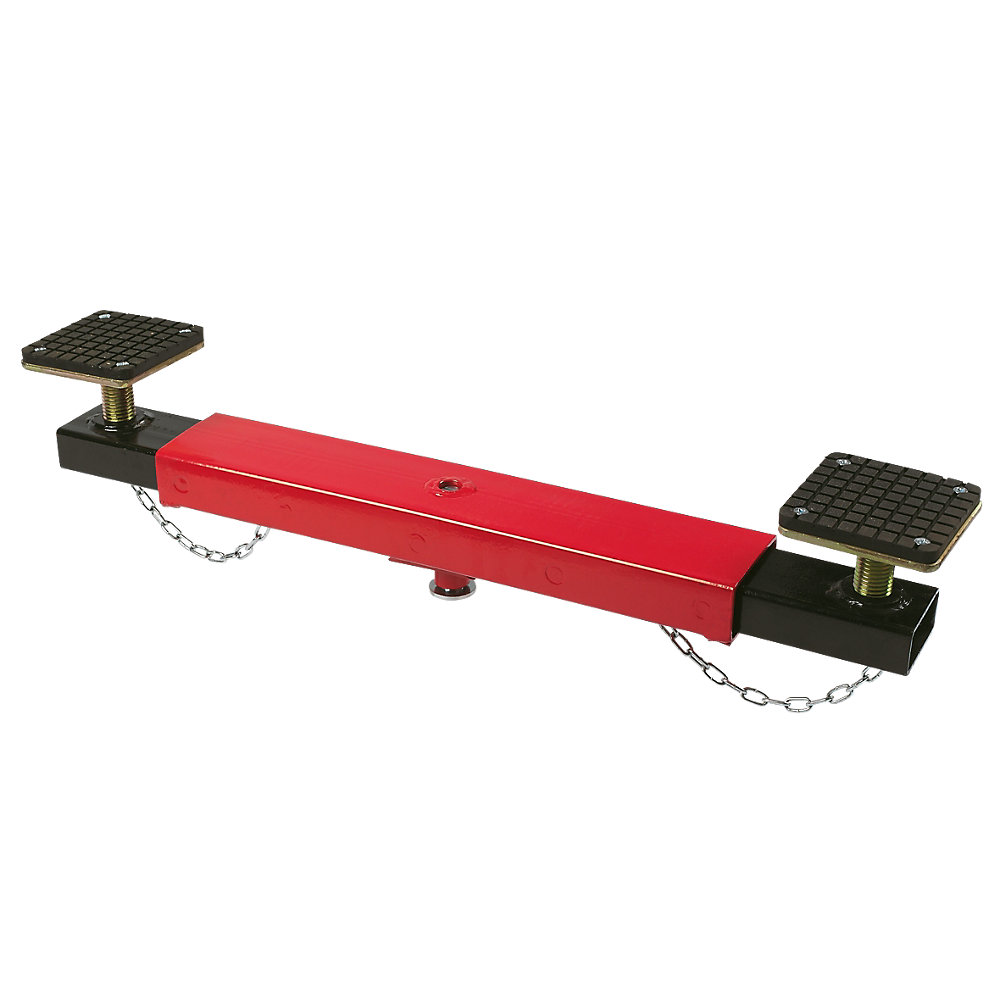
\includegraphics[width=150px]{./images/beamjack.jpg}
\caption{\label{fig:-Beam-Jack}Beam Jack}
\end{figure}



\section{Alternate Loadcell solutions}
\label{sec-2}

From looking at how the results of readings vary depending on load cell and there is no linearity between the environment 
and balance reading at the time. 

Replacing the load cells seems like a sensible path at this stage.  

\subsection{Building our own loadcell}
\label{sec-2-1}

The alternate to trying to get our current load cells to work is an attempt at constructing our own load cells. There are two options 
for this both will most likely costing a lot more than the aforementioned solution of a lifting mechanism. 

\subsubsection{Hanging Basket}
\label{sec-2-1-1}

S-Beam load cells are designed for constant load, they are used often in construction of bridges and buildings where a joint will be under constant strain
and it is important for this to be monitored over time for changes. 

For us to benefit from this we would require a hanging basket to hold plants 
\begin{figure}[htb]
\centering
\includegraphics[width=150px]{./images/basket.png}
\caption{\label{fig:Hanging-Basket}Example of a hanging basket}
\end{figure}


\begin{enumerate}
\item Suggested Cell
\label{sec-2-1-1-1}
The omega LCM101 can handle 10kg of force but can come in models supporting up-to 10,000 kg
Price: £222
\begin{figure}[htb]
\centering
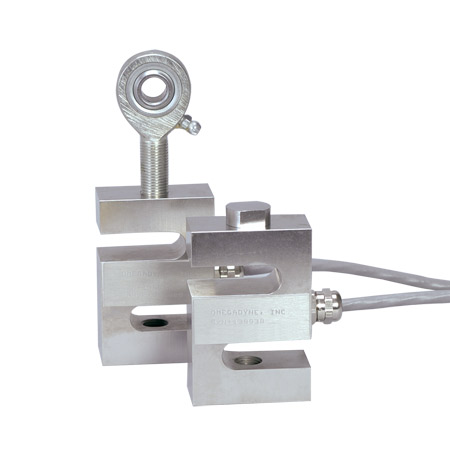
\includegraphics[width=120px]{./images/sbeam.jpg}
\caption{\label{fig:S-Beam}S-Beam load cell}
\end{figure}
\end{enumerate}

\subsubsection{Beam}
\label{sec-2-1-2}
The omega LCM501 cell has very high accuracy and Omega has assured me that this load cell has very little
creep factor and would be suitable for what we want to do. 

Price: £249
\begin{figure}[htb]
\centering
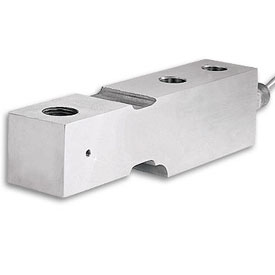
\includegraphics[width=150px]{./images/beam.jpg}
\caption{\label{fig:Beam}Beam load cell}
\end{figure}

\subsubsection{Additional info on constructing loadcells}
\label{sec-2-1-3}

The additional issue with building our own is that we would need to source amplifier boards 
e.g \href{http://www.omega.co.uk/pptst/TXDIN1600S.html}{Expensive one}, or \href{https://www.proto-pic.co.uk/sparkfun-load-cell-amplifier-hx711.html?gclid\%3DCjwKEAjw5vu8BRC8rIGNrqbPuSESJADG8RV0786RXJOCIUPOVZj8QwYWbhOZYXY1rYzwlpp2wl3cfRoCgTTw_wcB}{this cheap one}. 

Moreover we would need to worry about casing and could still face the same creep problem as before, 
without building prototypes we couldn't be sure to their reliability. 

\subsection{Purchase options}
\label{sec-2-2}

\subsubsection{Phenospex}
\label{sec-2-2-1}

\begin{figure}[htb]
\centering
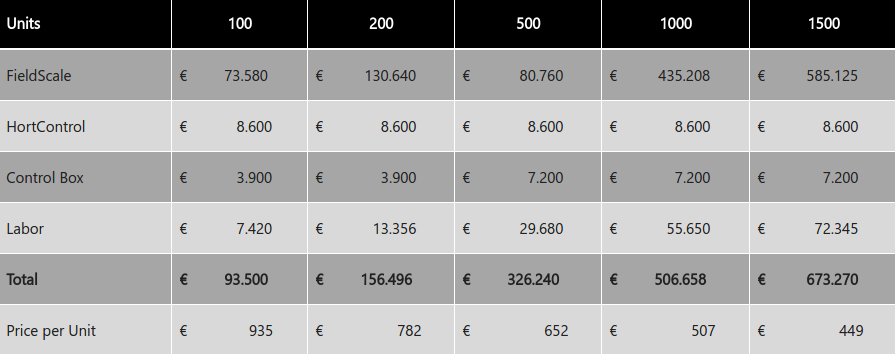
\includegraphics[width=.9\linewidth]{./images/price.png}
\caption{\label{fig:Phenospex-prices}Phenospex quotes}
\end{figure}


\subsubsection{Mettler Toledo PL6001E}
\label{sec-2-2-2}

Price: £600\textasciitilde{} per balance

The other option are these scales which I have been assured can do dynamic, continuous weighing. 
\href{http://uk.mt.com/dam/P5/labtec/03_Precision_Balances/12_PL-E/03_Documentation/02_Datasheet/DS_PL-E_Precision_EN.pdf}{PDF of this model }

\begin{figure}[htb]
\centering
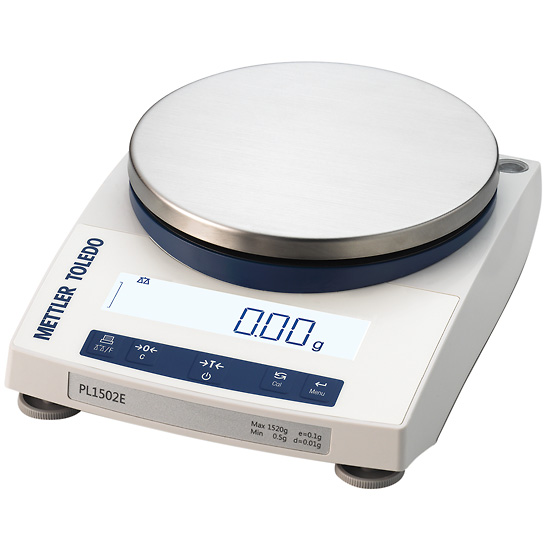
\includegraphics[width=120px]{./images/scale.jpg}
\caption{\label{fig:MT-Scale}Mettler Toledo scale}
\end{figure}
% Emacs 25.1.50.2 (Org mode 8.2.10)
\end{enumerate}
\end{document}
